\documentclass[12pt]{article}

% Packages
\usepackage{hyperref}
\usepackage{amsmath}
\usepackage{amsfonts}
\usepackage{amssymb}
\usepackage{algorithm2e}
\usepackage[noend]{algpseudocode}
\usepackage{listings}
\usepackage{xcolor}
\usepackage{float}
\usepackage{multicol}
\usepackage[a4paper, margin=1in]{geometry}
\usepackage{tikz}
\usepackage{tikz-cd}
\usepackage{graphicx}
\usetikzlibrary{shapes,arrows,positioning,calc,shapes.geometric}

% Configure listings package for code
\lstset{
    breaklines=true,
    breakatwhitespace=true,
    basicstyle=\ttfamily\small,
    columns=flexible,
    frame=single,
    numbers=left,
    numberstyle=\tiny,
    showstringspaces=false,
    tabsize=2
}

\begin{document}

\title{Building an Oracle Network for Ethereum to Leverage Large Language Models}
\author{Madhukara S. Holla (Team 2)}
\date{}
\maketitle

\section{Introduction}
Smart contracts on blockchain networks are inherently limited to deterministic on-chain data. This limitation poses a challenge when integrating with Large Language Models (LLMs), which provide valuable but non-deterministic outputs. This project implements a decentralized oracle network that enables Ethereum smart contracts to securely interact with LLMs while maintaining consensus across the network.

\section{Problem Definition}
Smart contracts are deterministic by design to ensure consensus across blockchain nodes. This determinism limits their ability to interact with external, dynamic, and non-deterministic systems like LLMs. The key challenges include:

\begin{itemize}
    \item \textbf{Achieving Consensus:} LLMs generate probabilistic outputs, making it difficult for blockchain nodes to agree on a single result.
    \item \textbf{Ensuring Verifiability:} Blockchain systems rely on transparent and immutable data. Integrating LLMs requires mechanisms to verify and log their outputs in a trustless environment.
\end{itemize}

\section{System Architecture}
The system implements a decentralized oracle network that enables smart contracts to access LLM capabilities while maintaining consensus on non-deterministic outputs. A high level system architecture diagram is provided in Appendix~\ref{appendix:arch} (Figure~\ref{fig:system-architecture}).

\subsection{Core Components}
\begin{itemize}
    \item \textbf{Decentralized Oracle Network:} A network of 7 nodes operates under a Practical Byzantine Fault Tolerance (PBFT) consensus mechanism to handle non-deterministic LLM outputs.
    \item \textbf{Smart Contract Interface:} Solidity-based contracts deployed on the Polygon ZKEVM testnet facilitate the submission of queries to the oracle network and retrieval of responses.
    \item \textbf{Decentralized Storage:} The InterPlanetary File System (IPFS) stores interaction logs, with corresponding hash references maintained on-chain for verifiability.
    \item \textbf{Response Validation:} Semantic similarity scoring algorithms, implemented using cosine similarity, assess the consistency of LLM responses across oracle nodes.
\end{itemize}

\subsection{System Components and Implementation}
The system is implemented in Go and consists of the following key components, with specific implementation details and library usage:

\begin{itemize}
    \item \textbf{Oracle Node Component} (oracle/pkg/):
    \begin{itemize}
        \item Core PBFT implementation in \texttt{consensus/pbft.go}:
        \begin{itemize}
            \item Complete protocol implementation including normal operation, view change, and recovery
            \item Custom message handling using Go's native channels and mutexes
            \item SHA-256 for message digests (Go's \texttt{crypto/sha256})
            \item ECDSA signatures using Ethereum's \texttt{secp256k1} library
            \item State management using in-memory maps with periodic checkpointing
        \end{itemize}

        \item Network Communication:
        \begin{itemize}
            \item HTTP/WebSocket-based communication using Go's \texttt{net/http} package
            \item JSON message serialization for inter-node communication
            \item Static node configuration through config files (no dynamic discovery)
            \item TLS encryption for secure communication
        \end{itemize}

        \item LLM Integration:
        \begin{itemize}
            \item Direct OpenAI API integration using \texttt{go-openai} v1.36.0
            \item Response normalization using tokenization and embedding
            \item Cosine similarity calculation for response comparison
            \item Configurable similarity thresholds for consensus
        \end{itemize}
    \end{itemize}

    \item \textbf{Smart Contract Component} (contracts/):
    \begin{itemize}
        \item Single Solidity smart contract (v0.8.19):
        \begin{itemize}
            \item \texttt{Oracle.sol}: Implements the complete oracle functionality
            \begin{itemize}
                \item Request creation and fee handling
                \item Response submission with IPFS CID storage
                \item Request state tracking and verification
                \item Oracle node management and access control
            \end{itemize}
        \end{itemize}
        \item Integration with Ethereum-compatible networks
        \item Event emission for request and response tracking:
        \begin{itemize}
            \item RequestCreated: Emitted when new requests are submitted
            \item ResponseReceived: Emitted when consensus responses are stored
            \item OracleNodeRegistered/Removed: Emitted during oracle management
        \end{itemize}
    \end{itemize}

    \item \textbf{Agent Component} (agent/):
    \begin{itemize}
        \item LLM Request Processing:
        \begin{itemize}
            \item Prompt templating and validation
            \item Rate limiting and retry mechanisms
            \item Error handling and fallback strategies
        \end{itemize}
        \item Response Processing:
        \begin{itemize}
            \item Tokenization using OpenAI's \texttt{tiktoken} library for GPT-4
            \item Vector embeddings using OpenAI's text-embedding-ada-002 model
            \item Semantic similarity computation using cosine distance between embeddings
            \item Response format standardization with JSON schema validation
        \end{itemize}
    \end{itemize}

    \item \textbf{Listener Component} (scripts/):
    \begin{itemize}
        \item Event Monitoring:
        \begin{itemize}
            \item Direct blockchain interaction using \texttt{go-ethereum} v1.13.5
            \item Event filtering and parsing using \texttt{go-ethereum/accounts/abi}
            \item Block polling with configurable intervals (5 seconds)
            \item Automatic block range tracking and event filtering
        \end{itemize}
        \item Response Management:
        \begin{itemize}
            \item IPFS integration using Pinata API
            \item Secure file pinning with JWT or API key authentication
            \item Automatic gas price optimization using \texttt{SuggestGasPrice}
            \item Concurrent request handling with Go contexts and channels
        \end{itemize}
    \end{itemize}
\end{itemize}

All components are containerized using Docker with Alpine Linux base images for minimal footprint. Configuration is managed through environment variables and JSON config files, with sensitive data (API keys, private keys) handled through secure environment variables.

\subsection{LLM Response Consensus}
The system handles non-deterministic LLM outputs through a semantic similarity-based consensus mechanism:

\begin{itemize}
    \item \textbf{Response Collection:}
    \begin{itemize}
        \item Each node independently queries the LLM with the same prompt
        \item Responses are normalized by removing whitespace and formatting
        \item Each node broadcasts its response to all other nodes
    \end{itemize}

    \item \textbf{Similarity Calculation:}
    \begin{itemize}
        \item Each node computes pairwise cosine similarity between all received responses
        \item Responses are converted to vector representations using word embeddings
        \item Similarity score $S_{ij}$ between responses $i$ and $j$ is calculated as:
        \[ S_{ij} = \frac{\vec{v_i} \cdot \vec{v_j}}{|\vec{v_i}| |\vec{v_j}|} \]
        where $\vec{v_i}$ and $\vec{v_j}$ are the vector representations
    \end{itemize}

    \item \textbf{Consensus Process:}
    \begin{itemize}
        \item Each node identifies the response with highest average similarity to all others
        \item A response is considered valid if its similarity score exceeds threshold $\tau$ (set to 0.8)
        \item Nodes only commit if 2f+1 nodes agree on a response meeting the threshold
        \item The leader node (current primary) selects the final response from the valid set
    \end{itemize}

    \item \textbf{Response Selection:}
    \begin{itemize}
        \item Leader chooses the response with highest average similarity score
        \item Selected response must have been validated by at least 2f+1 nodes
        \item If no response meets criteria, the consensus round fails
        \item Failed rounds trigger a new round of LLM queries
    \end{itemize}
\end{itemize}

This approach ensures that even with non-deterministic LLM outputs, the network can achieve consensus on semantically equivalent responses while filtering out significantly divergent ones.

\section{PBFT Implementation}
Our implementation extends the traditional PBFT protocol to handle non-deterministic LLM outputs. The complete algorithm is provided in Algorithm \ref{alg:pbft} in the Appendix. The implementation includes:

\begin{itemize}
    \item \textbf{Message Structure and State Management:}
    \begin{itemize}
        \item Messages are structured to include type, sender ID, view number, sequence number, digest, and data (see Listing \ref{lst:message-struct})
        \item Each PBFT instance maintains state including current view, sequence number, and message buffers
        \item Thread-safe operations using mutex locks for concurrent message handling
        \item Message types include PrePrepare, Prepare, Commit, and ViewChange
    \end{itemize}

    \item \textbf{Cryptographic Components:}
    \begin{itemize}
        \item SHA-256 for message digest computation (see Listing \ref{lst:digest})
        \item Message verification includes sender validation, sequence number checks, and view number validation
        \item ECDSA (secp256k1) for digital signatures using Ethereum's crypto libraries
        \item Digest verification ensures message integrity throughout consensus phases
    \end{itemize}

    \item \textbf{Consensus Protocol Flow:}
    \begin{itemize}
        \item Pre-prepare phase: Leader computes digest and broadcasts proposal
        \item Prepare phase: Nodes validate and broadcast prepare messages after digest verification
        \item Commit phase: Nodes wait for 2f+1 prepare messages before committing
        \item Each phase includes message validation and state updates
        \item Messages are tracked using sequence numbers for ordering
        \item Detailed algorithm provided in Appendix (see Algorithm \ref{alg:pbft})
    \end{itemize}

    \item \textbf{View Change Protocol:}
    \begin{itemize}
        \item Triggered by view change timeout or leader failure detection
        \item Nodes broadcast view change messages with current state (see Listing \ref{lst:viewchange})
        \item New view starts when 2f+1 view change messages are received
        \item View change includes state transfer and message cleanup
        \item Leader selection based on view number modulo number of nodes
    \end{itemize}

    \item \textbf{State Management and Recovery:}
    \begin{itemize}
        \item Periodic checkpoints every 100 sequences (see Listing \ref{lst:checkpoint})
        \item Garbage collection of old messages and checkpoints
        \item State includes prepare messages, commit messages, and view change messages
        \item Recovery possible through checkpoint restoration
        \item Message cleanup triggered after consensus or view changes
    \end{itemize}

    \item \textbf{Fault Tolerance:}
    \begin{itemize}
        \item Tolerates f Byzantine failures where f = (n-1)/3
        \item 7-node network configuration handles up to 2 Byzantine nodes
        \item Safety guaranteed through 2f+1 matching prepare messages
        \item Liveness ensured through view change protocol
        \item Message validation prevents equivocation attacks
    \end{itemize}
\end{itemize}

\section{Results}
The implementation of the decentralized oracle network achieved the following:

\begin{itemize}
    \item \textbf{Consensus Achievement:} The oracle network successfully achieved consensus with up to $f = \lfloor(n-1)/3\rfloor$ Byzantine nodes, even with non-deterministic LLM outputs.
    \item \textbf{Efficient Storage:} Using IPFS for off-chain storage minimized on-chain data footprint, reducing gas costs while maintaining verifiability through hash references.
    \item \textbf{Verifiable Logs:} All LLM interactions were logged in an immutable and verifiable manner, ensuring transparency and auditability.
    \item \textbf{Performance Metrics:} The system demonstrated a sub-30-second response time for LLM queries and effectively handled multiple concurrent requests using its Dockerized architecture.
    \item \textbf{Blockchain Integration:} The deployed smart contracts on the Polygon ZKEVM testnet reliably logged IPFS CIDs, enabling end-to-end traceability of oracle responses.
\end{itemize}

\section{Limitations}
The current implementation has the following limitations:
\begin{itemize}
    \item \textbf{No Recovery Mechanism for PBFT Nodes:} The system does not implement recovery protocols for failed or disconnected nodes within the PBFT network.
    \item \textbf{No Peer Discovery:} Nodes must be manually configured as the system lacks automated peer discovery mechanisms.
    \item \textbf{No Staking by the Nodes:} Nodes do not stake any assets, resulting in a lack of economic incentives or "skin in the game" for honest participation.
\end{itemize}

\section{Conclusion}
This project successfully addresses the challenges of integrating non-deterministic LLM outputs into Ethereum smart contracts. By implementing a decentralized oracle network with robust PBFT consensus, cost-efficient storage using IPFS, and verifiable logging on the Polygon ZKEVM testnet, the system enables blockchain applications to harness the potential of AI-driven insights.

\begin{thebibliography}{9}

    \bibitem{castro1999practical}
    Castro, M., \& Liskov, B. (1999).
    \textit{Practical Byzantine fault tolerance}.
    In OSDI '99: Proceedings of the Third Symposium on Operating Systems Design and Implementation.

    \bibitem{castro2002practical}
    Castro, M., \& Liskov, B. (2002).
    \textit{Practical Byzantine fault tolerance and proactive recovery}.
    ACM Transactions on Computer Systems.

    \bibitem{kotla2007zyzzyva}
    Kotla, R., Alvisi, L., Dahlin, M., Clement, A., \& Wong, E. (2007).
    \textit{Zyzzyva: speculative byzantine fault tolerance}.
    ACM SIGOPS Operating Systems Review.

    \bibitem{yin2019hotstuff}
    Yin, M., Malkhi, D., Reiter, M. K., Gueta, G. G., \& Abraham, I. (2019).
    \textit{Hotstuff: BFT consensus with linearity and responsiveness}.
    In Proceedings of the ACM Symposium on Principles of Distributed Computing.

\end{thebibliography}

\clearpage
\appendix
\section{System Architecture Diagram}\label{appendix:arch}
\begin{figure}[H]
\centering
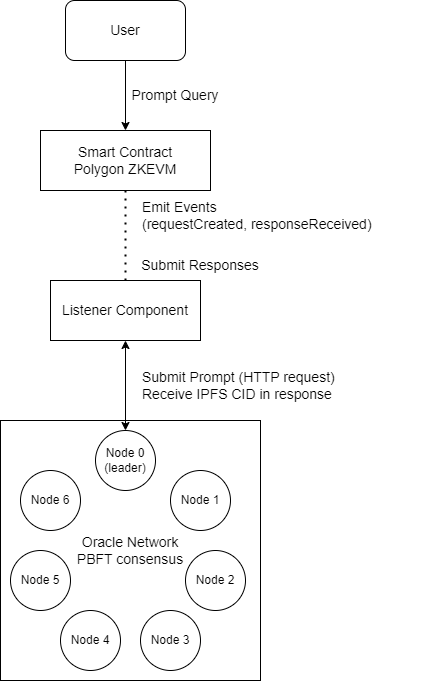
\includegraphics[width=0.5\textwidth]{oracle_network.png}
\caption{System Architecture Overview showing the interaction between smart contracts, oracle nodes in a PBFT consensus mechanism}
\label{fig:system-architecture}
\end{figure}

\clearpage
\section{PBFT Algorithm Details}\label{sec:algo}
Our PBFT implementation follows Algorithm \ref{alg:pbft}, which extends the traditional PBFT protocol to handle non-deterministic LLM outputs.

\begin{algorithm}[H]
\SetAlgoLined
\caption{PBFT Consensus for LLM Oracle Network}\label{alg:pbft}
Initialize: $view \leftarrow 0$, $sequence \leftarrow 0$, $f \leftarrow \lfloor(n-1)/3\rfloor$\;
\BlankLine
\SetKwProg{Fn}{Function}{:}{}
\Fn{NormalOperation(request)}{
    \If{$isLeader$}{
        $digest \leftarrow \text{SHA256}(request)$\;
        Broadcast $\langle\text{PRE-PREPARE}, view, sequence, digest, request\rangle$\;
    }
}
\BlankLine
\Fn{HandlePrePrepare(msg)}{
    \If{$\text{ValidMessage}(msg) \land \text{ValidDigest}(msg)$}{
        Store $msg$ in $prepareMessages[sequence]$\;
        Broadcast $\langle\text{PREPARE}, view, sequence, digest\rangle$\;
    }
}
\BlankLine
\Fn{HandlePrepare(msg)}{
    \If{$\text{ValidMessage}(msg)$}{
        Store $msg$ in $prepareMessages[sequence]$\;
        \If{$|prepareMessages[sequence]| \geq 2f + 1$}{
            Broadcast $\langle\text{COMMIT}, view, sequence, digest\rangle$\;
        }
    }
}
\BlankLine
\Fn{HandleCommit(msg)}{
    \If{$\text{ValidMessage}(msg)$}{
        Store $msg$ in $commitMessages[sequence]$\;
        \If{$|commitMessages[sequence]| \geq 2f + 1$}{
            $response \leftarrow \text{GetConsensusResponse}()$\;
            $\text{ExecuteConsensus}(sequence, response)$\;
            $sequence \leftarrow sequence + 1$\;
        }
    }
}
\BlankLine
\Fn{ViewChange(newView)}{
    Broadcast $\langle\text{VIEW-CHANGE}, newView, sequence, state\rangle$\;
    \If{$|viewChangeMessages[newView]| \geq 2f + 1$}{
        $view \leftarrow newView$\;
        $isLeader \leftarrow (nodeID \bmod n = view)$\;
        $\text{ResetState}()$\;
    }
}
\BlankLine
\Fn{GetConsensusResponse()}{
    $responses \leftarrow \text{CollectLLMResponses}()$\;
    $similarities \leftarrow \text{ComputeSemanticSimilarities}(responses)$\;
    \Return $\text{SelectMostSimilarResponse}(similarities)$\;
}
\end{algorithm}
\vspace{0.3cm}

\section{Implementation Details}\label{sec:impl}
\subsection{PBFT Message Structure}
The PBFT consensus protocol uses a structured message format for all communication (see Listing \ref{lst:message-struct}):

\begin{lstlisting}[caption={PBFT Message Structure}, label={lst:message-struct}, language=Go]
// ConsensusMessage represents a message in the PBFT protocol
type ConsensusMessage struct {
    Type     MessageType // PrePrepare, Prepare, Commit, ViewChange
    NodeID   string     // Sender node identifier
    View     uint64     // Current view number
    Sequence uint64     // Message sequence number
    Digest   []byte     // Message digest (SHA-256)
    Data     []byte     // Actual message content
}

// PBFT represents a PBFT consensus instance
type PBFT struct {
    mu                 sync.RWMutex
    nodeID             string
    nodes              []string
    privateKey         *ecdsa.PrivateKey
    networkManager     *NetworkManager
    timeout            time.Duration
    viewChangeTimeout  time.Duration
    checkpointInterval uint64

    // State
    view              uint64
    sequence          uint64
    state             PBFTState
    isLeader          bool
    lastCheckpoint    []byte
    lastCheckpointSeq uint64

    // Messages
    prepareMessages   map[uint64]map[string]*ConsensusMessage
    commitMessages    map[uint64]map[string]*ConsensusMessage
    viewChangeMsgs    map[uint64]map[string]*ConsensusMessage
    checkpoints       map[uint64][]byte
    consensusReached  map[uint64]bool
}
\end{lstlisting}

\clearpage
\subsubsection{Message Digest and Verification}
The system uses SHA-256 for message digest computation and verification (see Listing \ref{lst:digest}):

\begin{lstlisting}[caption={Message Digest Implementation}, label={lst:digest}, language=Go]
func (p *PBFT) computeDigest(data []byte) []byte {
    hash := sha256.Sum256(data)
    return hash[:]
}

func (p *PBFT) validateMessage(msg *ConsensusMessage) error {
    if msg == nil {
        return ErrInvalidMessage
    }

    // Validate sender
    senderValid := false
    for _, node := range p.nodes {
        if node == msg.NodeID {
            senderValid = true
            break
        }
    }
    if !senderValid {
        return ErrInvalidSender
    }

    // Validate sequence number
    if msg.Sequence < p.sequence-1 && p.sequence > 1 {
        return ErrInvalidSequence
    }

    // Validate view number
    if msg.View < p.view-1 && p.view > 1 {
        return ErrInvalidView
    }

    return nil
}
\end{lstlisting}

\clearpage
\subsubsection{View Change Protocol}
The view change protocol ensures liveness when the leader fails (see Listing \ref{lst:viewchange}):

\begin{lstlisting}[caption={View Change Implementation}, label={lst:viewchange}, language=Go]
func (p *PBFT) startViewChange(newView uint64) {
    p.mu.Lock()
    defer p.mu.Unlock()

    // Create view change message
    msg := &ConsensusMessage{
        Type:     ViewChange,
        NodeID:   p.nodeID,
        View:     newView,
        Sequence: p.sequence,
    }

    // Store view change message
    if _, exists := p.viewChangeMsgs[newView]; !exists {
        p.viewChangeMsgs[newView] = make(map[string]*ConsensusMessage)
    }
    p.viewChangeMsgs[newView][p.nodeID] = msg

    // Broadcast view change
    p.broadcast(msg)
}

func (p *PBFT) handleViewChange(msg *ConsensusMessage) {
    p.mu.Lock()
    defer p.mu.Unlock()

    // Store view change message
    if _, exists := p.viewChangeMsgs[msg.View]; !exists {
        p.viewChangeMsgs[msg.View] = make(map[string]*ConsensusMessage)
    }
    p.viewChangeMsgs[msg.View][msg.NodeID] = msg

    // Check if we have enough view change messages
    if len(p.viewChangeMsgs[msg.View]) >= 2*p.f+1 {
        p.changeView(msg.View)
    }
}
\end{lstlisting}

\clearpage
\subsubsection{Consensus Flow}
The complete consensus flow implementation (see Listing \ref{lst:consensus}):

\begin{lstlisting}[caption={Consensus Flow Implementation}, label={lst:consensus}, language=Go]
func (p *PBFT) ProposeValue(value []byte) error {
    if !p.isLeader {
        return fmt.Errorf("node is not the leader")
    }

    p.mu.Lock()
    defer p.mu.Unlock()

    // Compute message digest
    digest := p.computeDigest(value)

    // Create pre-prepare message
    msg := &ConsensusMessage{
        Type:     PrePrepare,
        NodeID:   p.nodeID,
        View:     p.view,
        Sequence: p.sequence,
        Digest:   digest,
        Data:     value,
    }

    // Store message for validation
    if _, exists := p.prepareMessages[p.sequence]; !exists {
        p.prepareMessages[p.sequence] = make(map[string]*ConsensusMessage)
    }
    p.prepareMessages[p.sequence][p.nodeID] = msg

    // Broadcast pre-prepare message
    return p.broadcast(msg)
}

func (p *PBFT) handlePrepare(msg *ConsensusMessage) {
    p.mu.Lock()
    defer p.mu.Unlock()

    // Initialize prepare messages map for this sequence
    if _, exists := p.prepareMessages[msg.Sequence]; !exists {
        p.prepareMessages[msg.Sequence] = make(map[string]*ConsensusMessage)
    }

    // Store prepare message
    p.prepareMessages[msg.Sequence][msg.NodeID] = msg

    // Check if we have enough prepare messages
    if len(p.prepareMessages[msg.Sequence]) >= 2*p.f {
        // Send commit message
        commit := &ConsensusMessage{
            Type:     Commit,
            NodeID:   p.nodeID,
            View:     msg.View,
            Sequence: msg.Sequence,
            Digest:   msg.Digest,
            Data:     msg.Data,
        }
        p.broadcast(commit)
    }
}
\end{lstlisting}

\clearpage
\subsubsection{Checkpoint and State Management}
Implementation of checkpointing and state management (see Listing \ref{lst:checkpoint}):

\begin{lstlisting}[caption={Checkpoint Implementation}, label={lst:checkpoint}, language=Go]
func (p *PBFT) makeCheckpoint() {
    if p.checkpointInterval == 0 {
        p.checkpointInterval = 100
    }

    if p.sequence%p.checkpointInterval == 0 {
        checkpoint := &struct {
            Sequence uint64
            State    []byte
        }{
            Sequence: p.sequence,
            State:    p.lastCheckpoint,
        }

        checkpointBytes, _ := json.Marshal(checkpoint)
        p.checkpoints[p.sequence] = checkpointBytes
        p.lastCheckpointSeq = p.sequence
    }
}

func (p *PBFT) cleanup(sequence uint64) {
    // Cleanup old prepare messages
    for seq := range p.prepareMessages {
        if seq < sequence {
            delete(p.prepareMessages, seq)
        }
    }

    // Cleanup old commit messages
    for seq := range p.commitMessages {
        if seq < sequence {
            delete(p.commitMessages, seq)
        }
    }

    // Cleanup old consensus reached flags
    for seq := range p.consensusReached {
        if seq < sequence {
            delete(p.consensusReached, seq)
        }
    }

    // Cleanup old checkpoints
    for seq := range p.checkpoints {
        if seq < sequence-p.checkpointInterval {
            delete(p.checkpoints, seq)
        }
    }
}
\end{lstlisting}

\end{document}
